\chapter{Encountered Issues}

\section{Impossibility to read value from the encoders}
\subsection{Issue}
Sometime it can happen that, even if the HSC are correctly set to read values from the encoders, they do not work.
\subsection{Solution}
This issue can be easily solved by deassembling and removing the encoder box from its slot and rotating by hand the pin of the motor. After that the encoder box can be assembled and put again in its slot.

\section{Sending array of values from Matlab to TIA Portal}
\subsection{Issue}
A problem that had to be solved during the environment setup for this project was related to the communication between Matlab and TIA Portal. When it was tried to send more than one byte from Matlab to TIA Portal, the values sent could not be read.

\subsection{Solution}
The problem was solved \cite{TIAPorta92:online} by disabling the option "optimized access" of the Data Block in TIA Portal. This option can be disabled by right-clicking on the Data Block object, selecting "properties", then selecting "attributes" in the "general" window and finally unchecking the correspondent box.

\section{Correctly formatting data to be sent from Matlab to TIA Portal}

\subsection{Issue}
Another encountered problem regarding the communication between Matlab and TIA Portal was to find the correct way to format data in Matlab in order to correctly read them in TIA Portal. In fact it happened that when it was firstly tried to send data, they were not properly read by TIA Portal.

\subsection{Solution}
This issue was solved by sending from TIA Portal to Matlab the same data that were expected to be received by TIA Portal. Then the values received by Matlab were read and sent back to TIA Portal, where they were finally correctly read. From this experience it was found that the problem can be related to two different factors:
\begin{itemize}
    \item an uncorrect offset between sequential data;
    \item a different representation of the same data type in the two softwares (for example little endian vs big endian).
\end{itemize}
The offset problem can be adjusted by putting the correct number of zeros between successive data, while the representation problem can be solved by trials and errors, trying to decode the values using different possible  common representations until the correct one is found.

\section{Connection Timeout in communication between Matlab and TIA Portal}
\subsection{Issue}
It can happens that, when one of the two softwares involved in the communication is waiting for some data coming from the other software, the connection timeout expires and the data are not received in time.
\subsection{Solution}
This problem can be easily solved by modifying the connection timeout property of the connection object created by Matlab. This operation can be easily done by simply assigning a greater value in seconds. Foe example, assuming that the connection object variable is named "t" and that the wanted timeout is 180 seconds, it can be set with the following line of code:
\begin{lstlisting}[style=htmlcssjs,caption={Set connection timeout},label=code1]
t.timeout = 180;
\end{lstlisting}

\section{Some variables do not store the correct value after system merker activation in TIA Portal}
\subsection{Issue}
It can happen that if some variables are stored in memory addresses like $MDx$, after the activation of system merkers the values in those variables are not the correct ones.

\subsection{Solution}
This problem can be solved easily by assigning to system merkers memory addresses like $My$, respecting the condition $y\neq x$, because the addresses indicated with $Mx$ or $MDx$ point to the same memory location, but they refers to different size: $Mx$ indicates the starting point $x$ with a one-byte size, while $MDx$ indicates the starting point $x$ with an entire-word size.

To set all the memory addresses that are needed for our purpose 16 bits are enough since the greatest value that we can reach is around 4000 for the rotational counter, that is reached when the counterclockwise rotation stops. Since with 16 bits it is possible to reach values up to 65535, the operational range is covered. For this purpose, in those variables definition is enough to use a MW type (Memory Word) that is a 16 bits variable. The MB variables (Memory Byte) or M variables (Memory bit), related to the same kind of operation, are then assigned in the corresponding memory area. A list of all the data type is reported in the Figure\ref{fig:memory_variable_type}.

\begin{figure}[!h]
\begin{center}
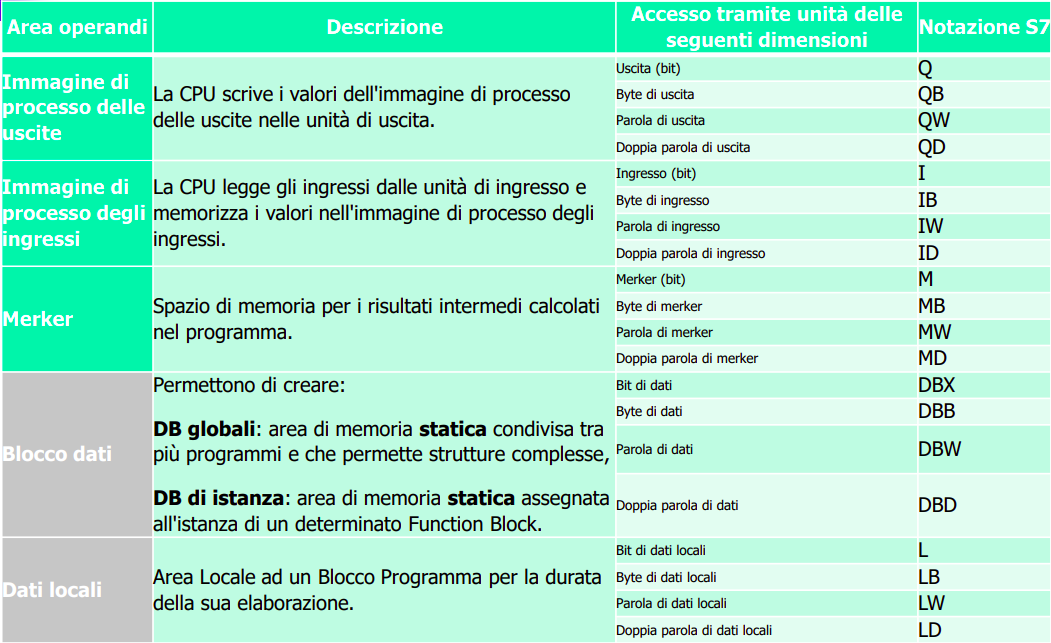
\includegraphics[width=\linewidth]{capitolo4/figure/memory_type_PLC.png}
\caption{Memory variable types in Siemens S7}
\label{fig:memory_variable_type}
\end{center}
\end{figure}
% FONTE: http://www.diit.unict.it/users/scava/dispense/II_270/PLCSiemens.pdf

In particular, in this project the memory addresses used are:


%\begin{table}[!htp]\centering
%\caption{Robot pinout %description}\label{tab:robot_pinout_description}
%\scriptsize
%\rowcolors{1}{}{tablelightgray}
%\begin{tabular}{lcccc}\toprule
%Terminal No. &Function &Pin Name &Robot %Input/Output \\\midrule
%1 &Power Supply (+) &24V DC &OUTPUT \\
%2 &Power Supply (+) &24V DC &OUTPUT \\
%3 &Power Supply (-) &0 &OUTPUT \\
%4 &Power Supply (-) &0 &OUTPUT \\
%5 &Fully Open Gripper &I1 &OUTPUT \\
%6 &Pulse Counter Gripper &I2 &OUTPUT \\
%7 &Fully Back Arm &I3 &OUTPUT \\
%8 &Pulse Counter Back Arm &I4 &OUTPUT \\
%9 &Fully Top Arm &I5 &OUTPUT \\
%10 &Fully Clockwise Arm &I6 &OUTPUT \\
%11 &Encoder Vertical Axis impulse 1 &B1 &OUTPUT \\
%12 &Encoder Vertical Axis impulse 2 &B2 &OUTPUT \\
%13 &Encoder Turnable Axis impulse 1 &B3 &OUTPUT \\
%14 &Encoder Turnable Axis impulse 2 &B4 &OUTPUT \\
%15 &Motor Gripper Open &Q1 &INPUT \\
%16 &Motor Gripper Close &Q2 &INPUT \\
%17 &Motor Arm Front &Q3 &INPUT \\
%18 &Motor Arm Back &Q4 &INPUT \\
%19 &Motor Arm Down &Q5 &INPUT \\
%20 &Motor Arm Up &Q6 &INPUT \\
%21 &Motor Rotation Clockwise &Q7 &INPUT \\
%22 &Motor Rotation Counter Clockwise &Q8 &INPUT \\
%\bottomrule
%\end{tabular}
%\end{table}

% Come merker di sistema clock zero
% Merker speciali 4: la connessione da 1 4

%ricordarsi questione pulsante premuto con movimento di 1 solo non si può incrementare soltanto di 1 il movimento, a causa della sensibilità del sensore
% come possibile soluzione: fare col clock